\documentclass{article}
\usepackage[utf8]{inputenc}
\usepackage{indentfirst}
\usepackage{listings}
\usepackage{natbib}
\usepackage{graphicx}
\lstset{
  language=bash,
  basicstyle=\ttfamily
}


\title{Nanako Search Engine}
\author{Linjiang Li}
\date{\today}

\begin{document} \maketitle
\section{Introduction}
		This program is for website search using website spider,TF-IDF and inverted index to achieve.\\ 
\indent You can crawl all the websites which can be reached from the URL you input.And run a small server on your PC. Then you can use browser to query the websites.\\
\indent It also supports the search for pdf files.
\section{Usage}
\emph{(The usage is for Windows OS, but you can still do similar operations on Linux)}
\subsection{}
	Python3($\geq$3.8.4) is recommended.

\subsection{}
To make sure you have the packages that will be used, run following command in your \emph{cmd} or \emph{bash}
\begin{lstlisting}
pip install flask
pip install jieba
pip install BeautifulSoup
pip install pdfminer
\end{lstlisting}

\subsection{}
This step is to make a database for following search\\
\indent You should run \emph{crawler.py}, \emph{parser.py}, \emph{index.py} one by one.\\
\indent (To avoid being banned by the website server,\emph{crawler.py} may take a lot of time.the rate of progress will be shown on the terminal)\\
\indent Here is an example for Windows: run following command in your \emph{cmd}
\begin{lstlisting}
crwaler.py
https://info.ruc.edu.cn (input the domain name you want to crawl)
parser.py
index.py
\end{lstlisting}

\subsection{}
This step is about how to use the search engine.\\
\indent Run \emph{routes.py}, then use your browser access \emph{https://127.0.0.1:5000/}\\
\indent And you will see the homepage
\begin{figure}[h!]
\flushleft

\includegraphics[width=12.5cm]{homepage.png}
\caption{Nanako search: Homepage}
\end{figure}
\\
\indent Then you can input your queries in the search bar, and access the result page.
\begin{figure}[h!]
\flushleft
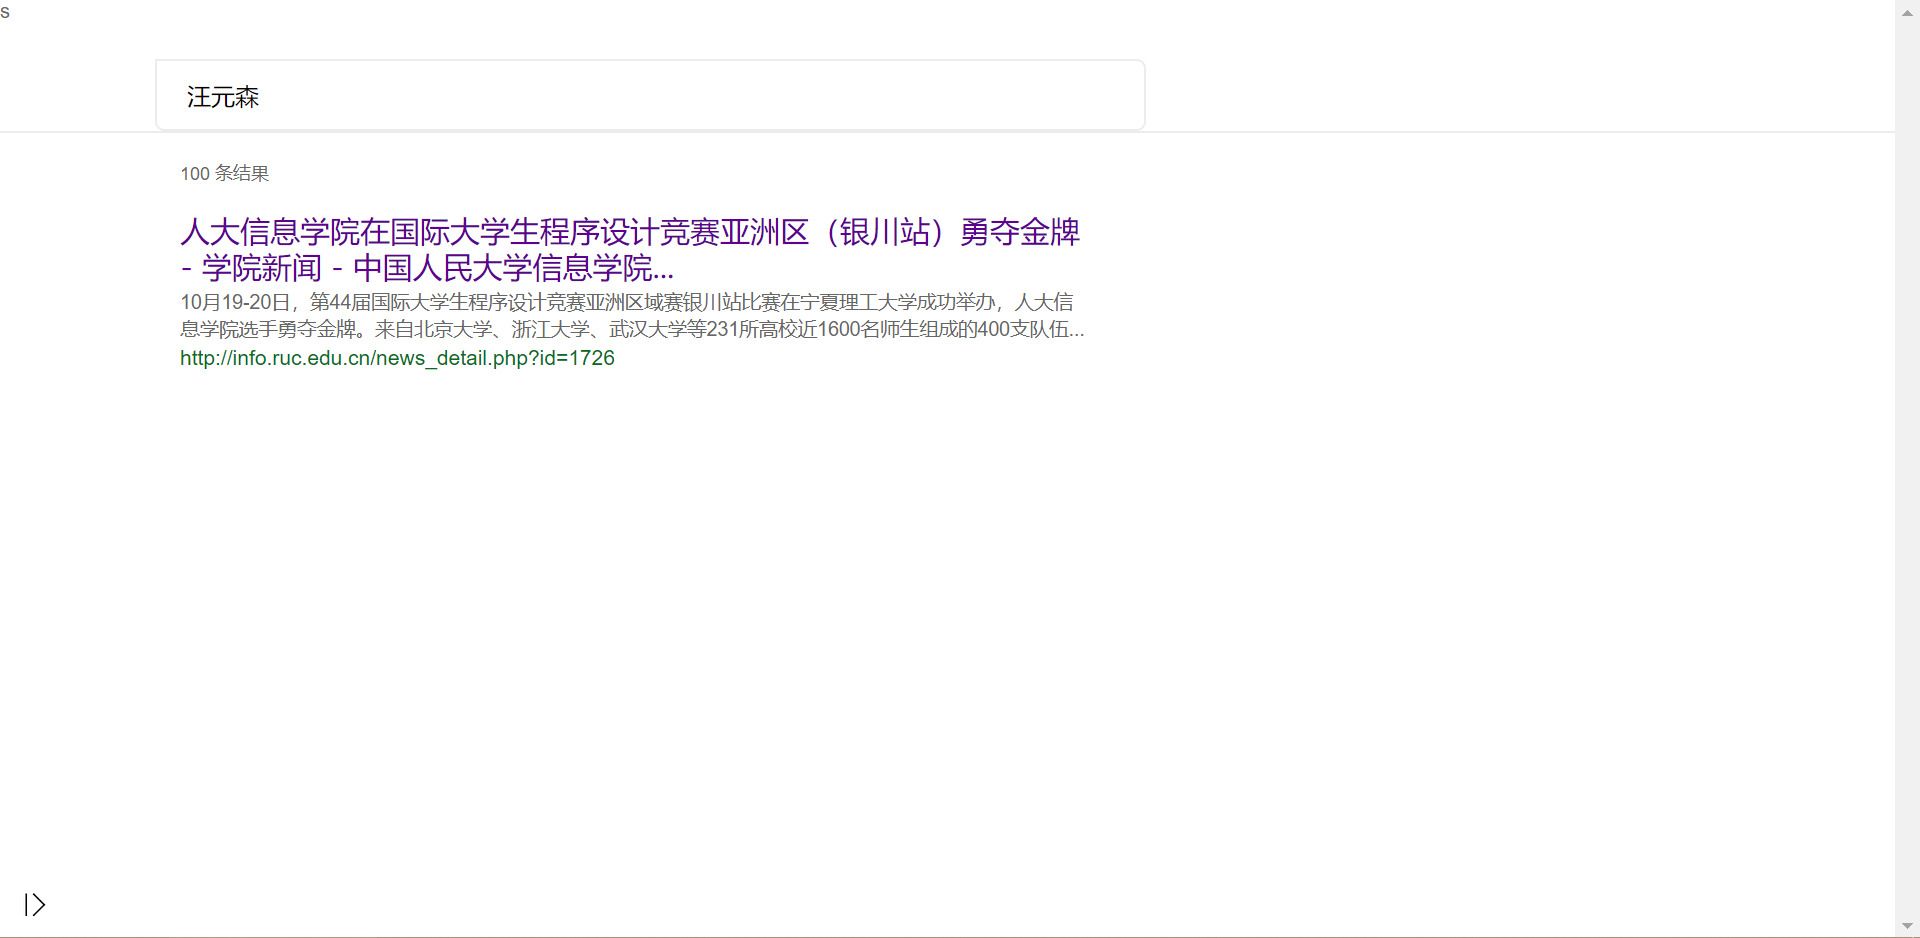
\includegraphics[width=12.5cm]{resultpage.png}
\caption{Nanako search: Resultpage}
\end{figure}
\section{Details}
\subsection{Crawler}
The crawler is implement with BeautifulSoup to get the URLs in label \emph{$<$herf$>$}\\
\indent Every accessable website will be downloaded in a file folder and numbered from 1 to n.\\
\indent content.xxx(file type,like php or pdf), url.txt,suf.txt will be in the file folder.
\begin{figure}[h!]
\flushleft
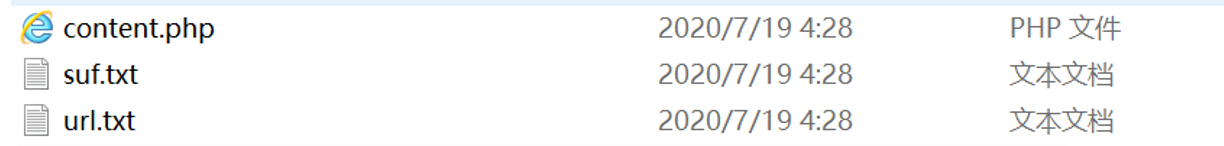
\includegraphics[width=12.5cm]{eg1.png}
\caption{Nanako search: Crawler}
\end{figure}
\indent Some urls will be ignored: the url with \emph{download?}, the url with \emph{mailto}, reduce \emph{index.php} in urls.

\subsection{Parser}
The crawler is implement with BeautifulSoup, pdfminer and jieba.\\
\indent The website content will be divided in to 3 fields: content,title and subtitle.\\
\indent For html, content.txt includes the content with \emph{$<$class=para$>$}, and \emph{$<$li$>$}.\quad subtitle.txt includes the content with \emph{$<$h1$>$}, \emph{$<$h2$>$}.\quad title.txt includes the content with \emph{$<$title$>$}.\\
\indent For html, it is difficult to divided the content into different fields.So all the content will be in content.txt\\

\indent After that, each field will be divded into single words by jieba.\\
\subsection{Index}
Undoubtedly, different fields enjoy different importance.So I use Fieldweight to measure its importance.(title = 10, subtitle = 2, content =1)\\
\indent $tf(word,document) = 1+log(\sum_{word\ in \ document}appeartimes \times Fieldweight)$ \\\\
\indent $idf(word) = 1+log(\frac{N}{\sum_{each\ document}tf(word,document)})\quad N = max(\sum_{each\ document}tf(word,document))$\\\\
\indent $score(query,document)= \sum_{word\ in\ query} tf(word,document)\times idf(word)$\\\\
\indent \emph{index.py} will return the highest 100 documents, and this step is implemented with muti-threads.
\section{Example}
Here shows some queries.\\
\begin{figure}[h!]
\flushleft
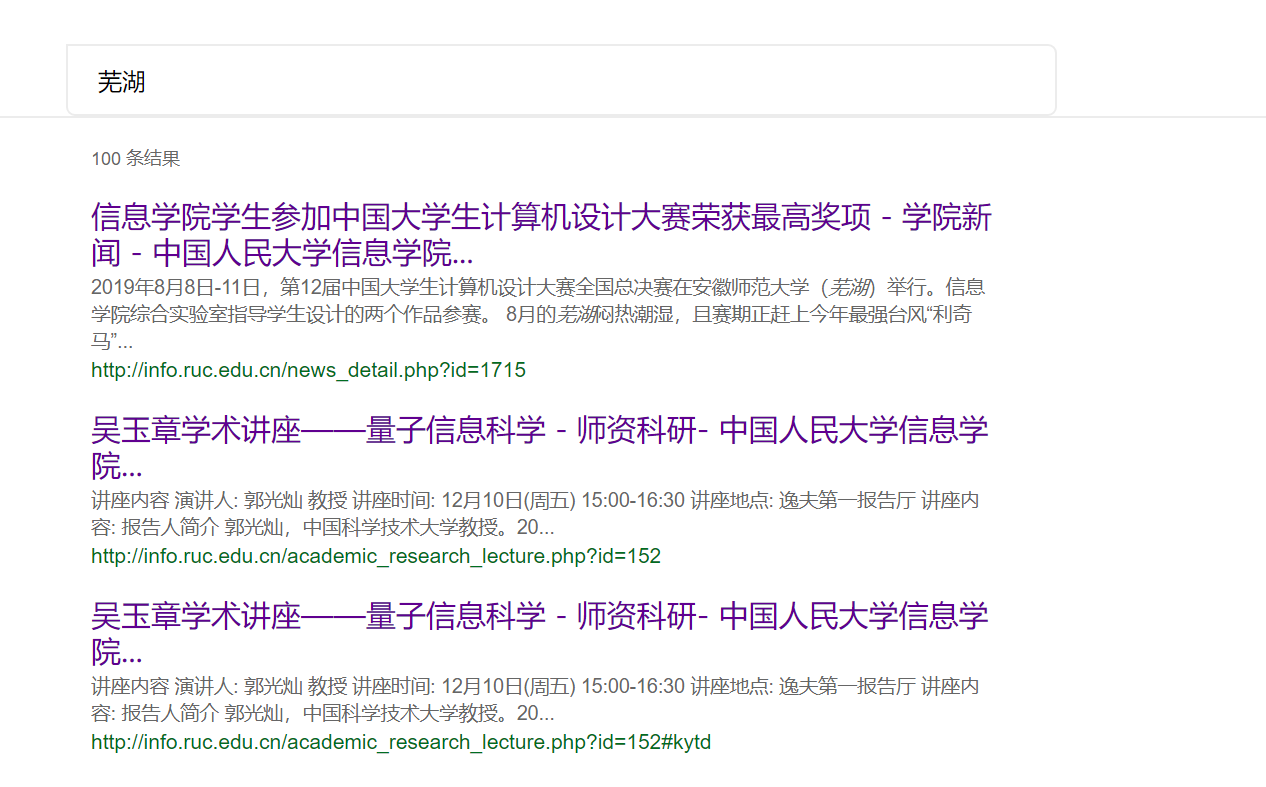
\includegraphics[width=10cm]{wuhu.png}
\caption{Example 1}
\end{figure}
\begin{figure}[h!]
\flushleft
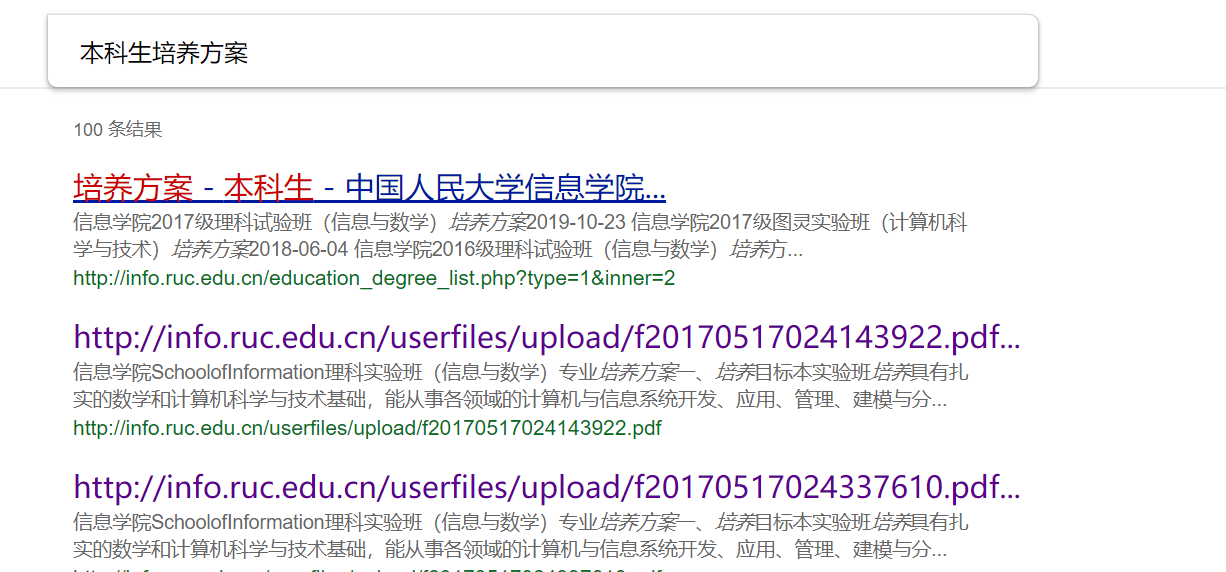
\includegraphics[width=12.5cm]{benkesheng.png}
\caption{Example 2}
\end{figure}
\begin{figure}[h!]
\flushleft

\includegraphics[width=12.5cm]{bks_detail.png}
\caption{pdf in Example 2}
\end{figure}
\begin{figure}[h!]
\flushleft

\includegraphics[width=15cm]{yuanzhang.png}
\caption{Example 3}
\end{figure}
\begin{figure}[h!]
\flushleft
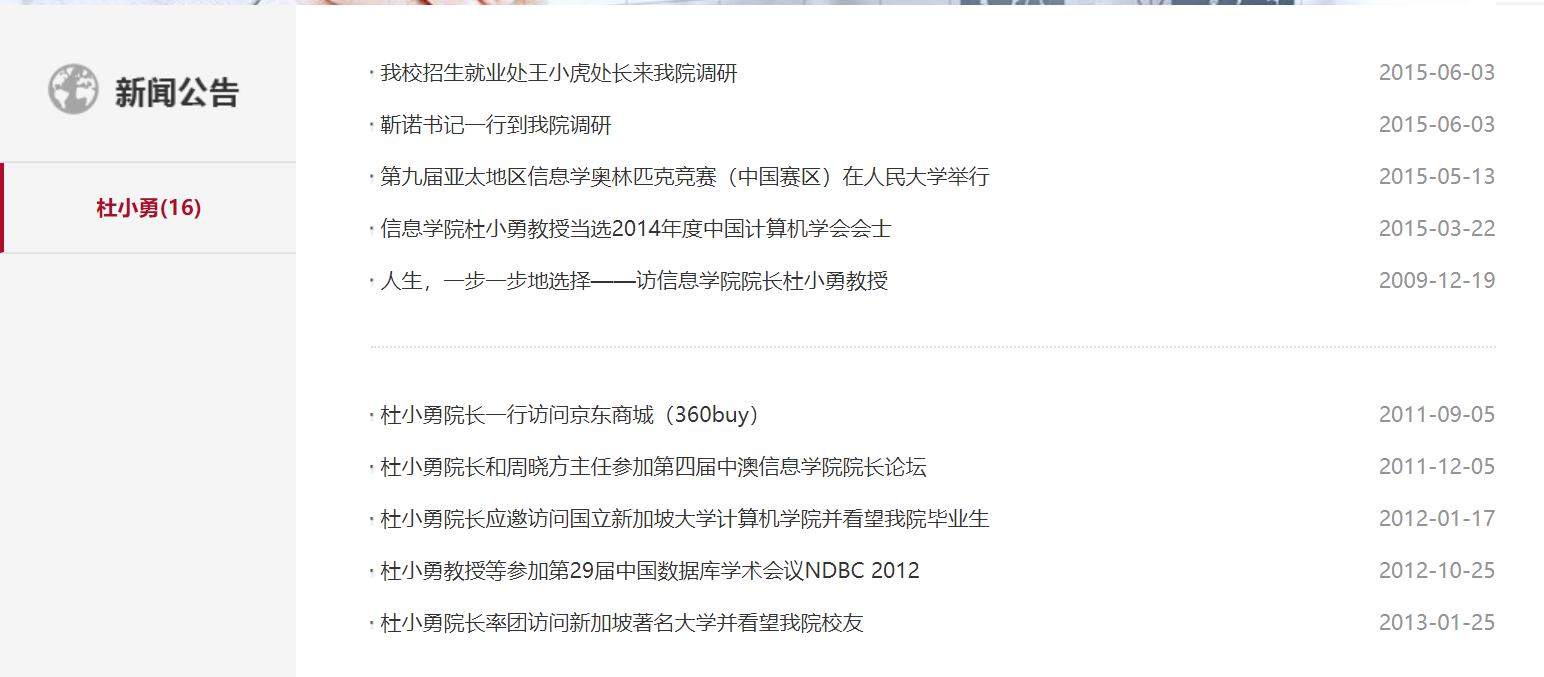
\includegraphics[width=12.5cm]{yuanzhang_detail.png}
\caption{Example 3 detail}
\end{figure}
\end{document}